% SandBlocks - Copyright 2024 Thiago M. de Oliveira. Solderpad Hardware License v2.1
% Script     : results.tex                                          Date: 2025.02.18
% Author     : Thiago M. de Oliveira <thiagomoraisee@gmail.com>
% Description: This chapter presents the synthesis results and test structure.

\section{Design Metrics and Validation}
\label{design_metrics_and_validation}

This section presents the design metrics and validation methodology for the \blockname\ block. It includes synthesis results, providing detailed information on area utilization, timing performance, and power consumption. Additionally, the verification strategy is described, outlining the test environment, applied stimuli, and coverage metrics used to ensure functional correctness. The goal is to demonstrate that the \blockname\ block meets the specified design requirements and operates reliably under defined conditions.

\subsection{Synthesis Results}

TBD

\begin{table}[h]	
    \centering
	\rowcolors{2}{white}{sandblue!10}
    \begin{tabular}{|c|c|c|c|c|}
		\arrayrulecolor{sandnavy!50}\hline
		\rowcolor{sandnavy!50}\hline
        % Columns labels:
        \textcolor{sandwhite}{Instance} &
        \textcolor{sandwhite}{Leakage}  &
        \textcolor{sandwhite}{Internal} &
        \textcolor{sandwhite}{Switch}   &
        \textcolor{sandwhite}{Total}    \\ \hline
        % Rows contents:
        \texttt{TBD} & $xx.xxx$ & $xx.xxx$ & $xx.xxx$ & $xx.xxx$ \\ \hline
	\end{tabular}
    \caption{\blockname's power results in $mW$.}
    \label{tab:power}
\end{table}

\begin{table}[h]	
    \centering
	\rowcolors{2}{white}{sandblue!10}
    \begin{tabular}{|c|c|c|c|c|}
		\arrayrulecolor{sandnavy!50}\hline
		\rowcolor{sandnavy!50}\hline
        % Columns labels:
        \textcolor{sandwhite}{Reg2Reg} &
        \textcolor{sandwhite}{In2Reg}  &
        \textcolor{sandwhite}{Reg2Out} &
        \textcolor{sandwhite}{In2Out}  &
        \textcolor{sandwhite}{ClockGate}    \\ \hline
        % Rows contents:
        $xx.xxx$ & $xx.xxx$ & $xx.xxx$ & $xx.xxx$ & $xx.xxx$ \\ \hline
	\end{tabular}
    \caption{\blockname's timing(slack) results in $ps$.}
    \label{tab:performance}
\end{table}

\begin{table}[h]	
    \centering
	\rowcolors{2}{white}{sandblue!10}
    \begin{tabular}{|c|c|c|c|c|}
		\arrayrulecolor{sandnavy!50}\hline
		\rowcolor{sandnavy!50}\hline
        % Columns labels:
        \textcolor{sandwhite}{Instance} &
        \textcolor{sandwhite}{Count}    &
        \textcolor{sandwhite}{Cell}     &
        \textcolor{sandwhite}{Net }     &
        \textcolor{sandwhite}{Total }   \\ \hline
        % Rows contents:
        \texttt{TBD} & $xxxx$ & $xx.xxx$ & $xx.xxx$ & $xx.xxx$ \\ \hline
	\end{tabular}
    \caption{\blockname's Area results in $\mu m^2$.}
    \label{tab:area}
\end{table}

\subsection{Validation}

The testbench structure is depicted in Figure \ref{fig:testbench}. It consists of three classes (in green) called Driver, Monitor, and Logger. The \textbf{Driver} is responsible for generating inputs based on the validation tests, while the \textbf{Monitor} captures the DUT's output and compares it with the reference (basically, a reference file). The \textbf{Logger} records and prints the test status (pass or fail) for each executed test. The same test task is is present in both Driver and Monitor with different purposes, and the testbench manages their parallel execution.

\begin{figure}[htb]
    \centering
    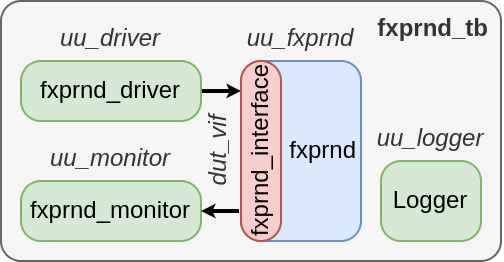
\includegraphics[width=9cm]{../doc/figs/fxprnd_testbench.png}
    \caption{Testbench structure for \blockname.}
    \label{fig:testbench}
\end{figure}

To run the testbench environment, the user must navigate to the \texttt{sandblocks/fxprnd/workspace/} directory and execute the \textbf{Makefile} using the command \texttt{make run} to perform the RTL simulation. The tests are self-checking and display the status of each stage in the report.
